%*******************************************************************************
% Macro per il documento corrente
%*******************************************************************************
\newcommand{\sharedPath}{../shared}
\newcommand{\doctitle}{Business Plan}

%*******************************************************************************
% Preambolo
%*******************************************************************************
\documentclass[a4paper,10pt,twoside]{book}

%*******************************************************************************
% Codifica e lingua
%*******************************************************************************
\usepackage[utf8x]{inputenc}
\usepackage[T1]{fontenc}
\usepackage[english,italian]{babel}
\usepackage{lmodern}
\usepackage{multirow}
\usepackage{amsmath,eurosym}
%*******************************************************************************
% Qualche macro utile a tutti
%*******************************************************************************
\newcommand{\docRoot}{..}
\newcommand{\inglese}[1]{\foreignlanguage{english}{\textit{#1}}}
\newcommand{\team}{\textsf{EtaBeta\,Software}\xspace}
\newcommand{\caName}{BPM-1.0\xspace}
\newcommand{\customer}{\textsf{Alpha\,\&\,Partners}\xspace}
\newcommand{\mktg}{\inglese{marketing}\xspace}
\newcommand{\bsn}{\inglese{business}\xspace}
\newcommand{\sw}{\inglese{software}\xspace}

%*******************************************************************************
% Figure e immagini
%*******************************************************************************
\usepackage{graphicx}
\graphicspath{{\docRoot/shared/pictures/}}

%*******************************************************************************
% Tabelle
%*******************************************************************************
\usepackage{booktabs}
\usepackage{array}

%*******************************************************************************
% Elenchi puntati personalizzati
%*******************************************************************************
\usepackage{enumitem}

%*******************************************************************************
% Landscape per ruotare le pagine
%*******************************************************************************
\usepackage{pdflscape}

%*************************************************
% Collegamenti intra- e intertestuali
%*************************************************
\usepackage{hyperref}
\hypersetup{%
    colorlinks=false,linktocpage=false,pdfborder={0 0 0},%
    pdfstartpage=1, pdfstartview=FitV,plainpages=false,%
    urlcolor=Black, linkcolor=Black,
    pdfcreator={pdfLaTeX},%
    pdfproducer={pdfLaTeX with hyperref package}%
}

%*************************************************
% Grafica vettoriale
%*************************************************
\usepackage{tikz}
\usetikzlibrary{shadows,arrows,shapes}

%*******************************************************************************
% Altri pacchetti
%*******************************************************************************
\usepackage{xspace} % per spazi condizionali extra
\usepackage{lastpage} % per sapere il numero totale di pagine
\usepackage{microtype} % qualche accorgimento tipografico

% *************************************************
% Intestazioni e piè di pagina personalizzati
% *************************************************
\usepackage{fancyhdr}

% stile normale
\fancypagestyle{normal}{
\fancyhead{}
\fancyhead[RE,LO]{
\sffamily\team
}
\fancyhead[LE,RO]{
\sffamily\leftmark
}
\renewcommand{\headrulewidth}{.4pt}
\cfoot{}
\fancyfoot[LE,RO]{\sffamily
  pag. \thepage{} di \pageref{LastPage}}
\fancyfoot[RE,LO]{\sffamily\doctitle}
\renewcommand{\footrulewidth}{.4pt}
}

% stile per gli indici
\fancypagestyle{toc}{
\fancyhead{}
\renewcommand{\headrulewidth}{0pt}
\cfoot{}
\fancyfoot[RO,LE]{\sffamily\thepage{}}
\fancyfoot[RE,LO]{\sffamily\doctitle{}}
\renewcommand{\footrulewidth}{.4pt}
}

\pagestyle{fancy}
\renewcommand{\sectionmark}[1]{\markboth{#1}{#1}}


%*******************************************************************************
% Inizio documento
%*******************************************************************************
\begin{document}

\pagestyle{empty}
\begin{center}

{\sffamily
Sviluppo e Gestione Progetti\\
a.a. 2012--2013
}

\vskip 1.5cm

{
\setlength{\fboxsep}{.2pt}
\fbox{
\includegraphics[width=\textwidth]{logo}}
}

\vskip .5cm

{\Huge\sffamily\bfseries
\team
}

\vskip 1.5cm

% titolo del progetto
{\Large\sffamily\bfseries
\caName
}

\vskip 1cm

% titolo del documento
\hrule
\vskip 10pt
{\Huge\scshape
\doctitle
}
\vskip 10pt
\hrule

\end{center}

\clearpage
\pagenumbering{roman} 

\tableofcontents{\thispagestyle{toc}}

\clearpage

\pagestyle{normal}
\pagenumbering{arabic}


% 1) NDA + DISCLAIMER
% 2) Executive summary
% 3) Descrizione generale della nostra azienda  (~3 pagine)
%   3.1) chi siamo
%   3.2) mission/vision
% 4) Mercato di riferimento: 
%   4.1) analisi della domanda (target di riferimento)
%   4.2) analisi del settore (modello delle 5 forze di Porter), SWOT
%   4.3) descrizione del problema + vantaggi competitivi che derivano dalla soluzione
% 5) Descrizione generale del progetto di sviluppo
%   5.1) descrizione di come è articolata soluzione
%       5.2.1) BPM per ottimizzare processi aziendali - ASPETTARE A SCRIVERLO!
%       5.2.2) corso su come utilizzare software BPM
%       5.2.3) acquisizione figure nuove, ad esempio un analista per capire necessità dei clienti
%       5.2.4) corsi di formazione in base alle carenze rilevate (ad esempio web design + accessibilità)
%        5.2.5) corso di Quality Assurance
%   5.2) risorse richieste per la realizzazione del progetto di sviluppo
%       5.3.1) tempistiche
%       5.3.2) risorse umane coinvolte
%       5.3.2) costi
%       5.3.3) prospettive di guadagno negli anni
\chapter{Note preliminari}

\section{Non-Disclosure Agreement}
Nel ricevere questo documento, vi impegnate a mantenere e garantire la massima riservatezza sulle informazioni ivi contenute, e su quelle di cui verrete a conoscenza, anche solo verbalmente, nel corso di eventuali ulteriori indagini e/o incontri, nonché a restituire immediatamente, su richiesta di \customer, tutto il materiale ricevuto senza trattenere alcuna copia.

Questo documento non dovrà essere fotocopiato, riprodotto o distribuito, per intero o in parte, né citato in documenti ufficiali, senza il preventivo consenso scritto di \customer.

\section{Disclaimer}
Il presente \inglese{business plan} è stato redatto secondo ipotesi, dati e indicazioni formulate e fornite da \customer, alla luce delle informazioni note, della situazione in essere e di quanto poteva essere ragionevolmente supposto, al momento della sua stesura.

Si precisa che, in conformità con l'incarico ricevuto, tali informazioni sono state assunte dai materiali redattori acriticamente, ovvero senza svolgere alcun controllo in merito alla correttezza, completezza e validazione dei dati e informazioni ricevute.

\chapter{Executive summary}\label{sec:summary}
% spiegare perché si dovrebbe investire nel progetto, qual è il suo scopo e perché è idealmente "unico"
% evitare slogan

\chapter{Informazioni sulla società}\label{sec:whoweare}

\section{Chi siamo}
\customer è un'azienda che opera nel settore della comunicazione e del marketing sia on-line che off-line. 
L'organizzazione si occupa in particolare di attività di \inglese{copywriter}, \inglese{mktg} tradizionale, grafica, e negli ultimi anni ha aperto le porte anche nei settori della comunicazione visiva e del \mktg on-line e \inglese{social}. In particolare, per quest'ultimo, le prospettive di mercato sono ottime e \customer prevede di aumentare gli investimenti in tale campo.

\customer è nata alla fine degli anni novanta come società di \inglese{marketing} tradizionale. Negli anni ha saputo rinnovarsi e rimanere al passo con un mercato sempre più dinamico e questa è stata la sua arma vincente.

Oggi, pur essendo un'azienda con un numero limitato di risorse, fattura circa  200.000,00 \text{\euro}.

\section{La nostra Mission}

\textit{``Nel mondo l'abito fa il monaco: il nostro obiettivo è farvi l'abito, il monaco lo dovete mettere voi!''}
%Sono riuscita a fuffare solo questo.... idee migliori?!


\chapter{Mercato di riferimento}
\section{Analisi della domanda}\label{sec:domanda}

Oggi il mercato si presenta molto dinamico, incline a continui cambiamenti e pieno di  \inglese{competitor}, in qualsiasi settore si operi. Il \mktg , in qualsiasi forma sia fatto, permette alle aziende di emergere rispetto ad altre e di reperire clienti, che costituiscono la fonte del guadagno di ogni organizzazione.

È  proprio per questo che, il \inglese{target} dei clienti delle aziende che operano nel settore del \mktg, come \customer , è molto vario e ampio. Qualsiasi azienda, di grandi o piccole dimensioni, può detenere interessi nel richiedere un intervento di consulenza \mktg con il fine di ampliare il suo \textit{portfolio} clienti.

Oggi, le aziende, puntano soprattutto al potenziamento del \mktg \inglese{online}. Infatti, negli ultimi anni, la crescita esponenziale del numero di utenti connessi alla rete ha moltiplicato le probabilità di reperire nuovi clienti e mantenere i contatti con quelli esistenti, proprio tramite \inglese{Internet}.

Molti e diversificati sono quindi i soggetti che in particolare nel Veneto necessitano del \inglese{know-how} e delle competenze trasversali che \customer mette a disposizione per il \inglese{digital} \mktg (in ambito \inglese{web} e \inglese{social}) e per l'ottimizzazione dei siti e del posizionamento nei motori di ricerca di questi ultimi.

\customer si colloca funzionalmente all'interno del tessuto piccolo e medio-industriale dell'area nordorientale del paese, con lo scopo di fungere idealmente da tramite dalla piccola realtà territoriale al mercato globale sia esso interno al paese che, grazie alla collaborazione con fornitori di servizi linguistici, esterno e internazionale.

\customer offre ai propri clienti un'ampia gamma di servizi che spaziano dall'elaborazione di strategie di \mktg al posizionamento sui motori di ricerca, dalla pubblicità \inglese{online} agli studi di \inglese{web analytics}, dalla creazione di contenuti all'internazionalizzazione di contenuti esistenti, fino agli aspetti \inglese{social} con la creazione di \inglese{blog} aziendali all'utilizzo di \inglese{Social Media Platforms} (\swname{Facebook}, \swname{LinkedIn}, \swname{Google+}, \swname{YouTube}).

Molte aziende decidono tuttavia di affidare le attività di \mktg a personale interno. Da uno studio del mercato nazionale, emerge che circa il 19\% delle aziende preferisce affidare il compito ad organizzazioni esterne specializzate \cite{picciaiola:indagine}.

Tale dato, riduce di molto il \inglese{target} effettivo di clienti che si rivolge ad aziende specializzate nel settore del \mktg.
Tuttavia, dallo stesso studio, emerge che circa il 97\% delle aziende utilizza il web come strumento di \mktg. È  proprio per questo motivo che, specializzandosi nel \mktg \inglese{on-line} e \inglese{social} le aziende operanti nel settore hanno maggior possibilità di acquisire tutti quei clienti che, pur affidando le attività di \mktg a settori interni,  mancano di preparazione ed esperienza nel campo web.

\section{Analisi del settore}
L'area del Nordest rappresenta indubbiamente un settore particolarmente critico dal punto di vista del \mktg \inglese{online}, dal momento che le PMI collocate in quest'area geografica non sempre sono in grado di sfruttare appieno le potenzialità offerte dalla rete per la commercializzazione dei prodotti e il lancio delle promozioni \cite[\itshape{}pag. 6 e succ.]{bassi:pmi}.

In particolare, lo studio evidenzia una scarsa efficacia nella comunicazione con il cliente, la diffusa incapacità di cogliere le nuovi occasioni di \bsn, i pochi collegamenti ai \inglese{social}, l'esiguità dei contenuti messi a disposizione in rete e una tendenza alla diffidenza nei confronti dell'\inglese{e-commerce}.

Uno scenario così configurato contiene, seppur allo stadio embrionale, importanti possibilità di espansione per il futuro, specialmente tenendo conto che l'\inglese{e-business} può essere volano per la ripresa dell'economia in un momento critico come quello attuale. È per questo motivo che \customer si andata specializzando sempre più nel \mktg digitale nel corso dei suoi vent'anni di presenza sul mercato.

È possibile avere una misura delle opportunità e della dimensione del margine di espansione presente nel settore tenendo conto del fatto che se nel nostro paese quasi nove utenti su dieci (89\%) si informano \inglese{online} su prodotti e \inglese{brand}, la percentuale di utenti che acquista su Internet si  arresta al 34\% ma con un potenziale di crescita non trascurabile: l'8\% dei \inglese{non-shopper} italiani si dichiara infatti disponibile ad aquistare \inglese{online} nei prossimi 12 mesi. A questo è da aggiungere il circolo virtuoso per
cui chi già acquistava nell’ultimo anno lo ha fatto più spesso e con maggior varietà \cite[\textit{pag.~3}]{contactlab:ecommerce}.

L'ambito del \mktg digitale mette in evidenza una serie di nuove tendenze il cui denominatore comune è la maggiore attenzione al (potenziale) cliente e una personalizzazione sempre più spinta dei messaggi e delle informazioni frutto delle campagne pubblicitarie tramite l'utilizzo dei dispositivi \inglese{mobile}.

Risulta infatti che un utente Internet su tre in Italia si connette abitualmente col proprio dispositivo mobile ma la percentuale di utilizza \inglese{smartphone} o \inglese{tablet} per acquistare \inglese{online} si arresta per ora solo al 20\%. Un dato già estremamente significativo per i \inglese{merchant} dell'\inglese{e-commerce} ma con enormi potenzialità di crescita, soprattutto se confrontato al 38\% rilevato in Germania e al 61\% rilevato in Gran Bretagna \cite{contactlab:ecommerce}. Il margine di espansione per il settore risulta evidente dal grafico riportato in \figurename~\ref{fig:potential}.

\begin{figure}[H]
  \centering
  \caption{Le opportunità di espansione per l'\inglese{e-commerce} in Italia.}
  \label{fig:potential}
  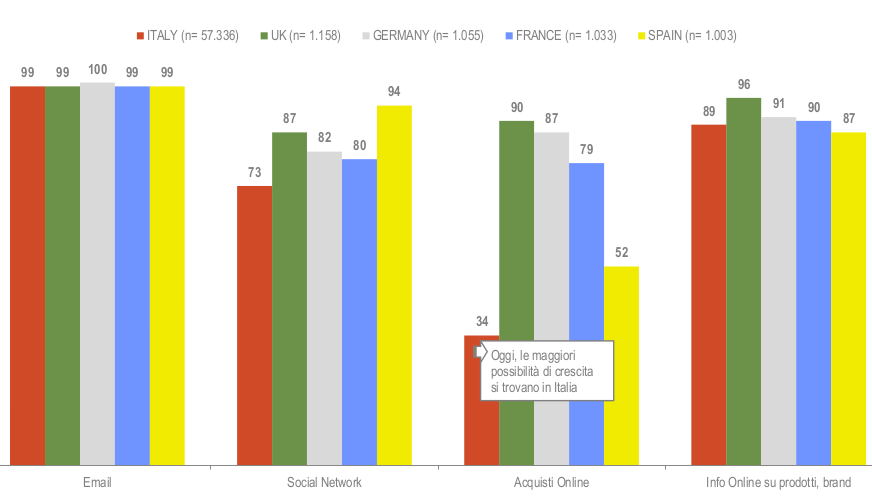
\includegraphics[width=.65\textwidth]{potential}
\end{figure}

L'entità della \inglese{profitability} del settore è evidente anche considerando l'andamento nell'ultimo anno (2013) di indicatori quali la frequenza degli acquisti \inglese{online}, la varietà dei prodotti/servizi acquistati e la somma totale spesa in acquisti \inglese{online} che mostrano un incremento, rispettivamente, del 63\%, 57\% e 55\% (\figurename~\ref{fig:potential2}).

\begin{figure}[H]
  \centering
  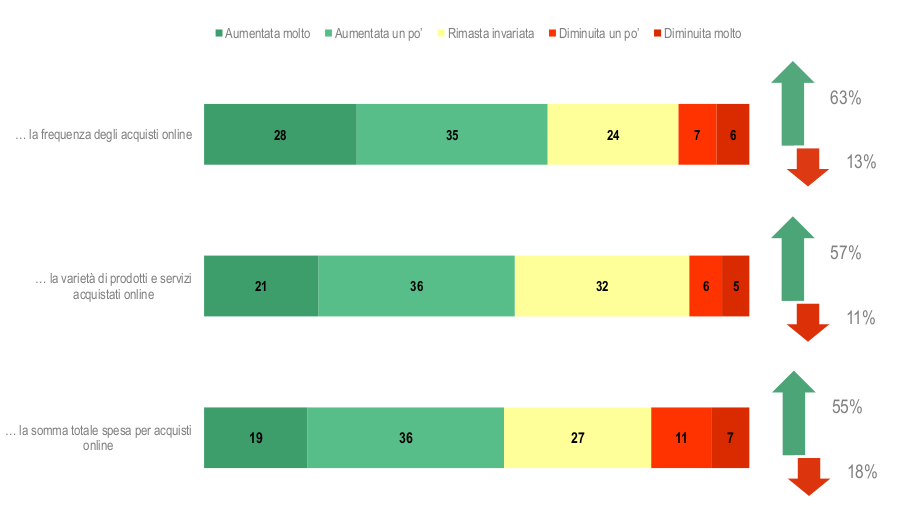
\includegraphics[width=.7\textwidth]{potential2}
  \caption{La tendenza dell'utilizzo di \inglese{e-commerce} nell'ultimo anno.}
  \label{fig:potential2}
\end{figure}

Grazie ai servizi di geolocalizzazione disponibili sui dispositivi \inglese{mobile}, ad esempio, è possibile da un lato raccogliere dati sui consumatori e dall'altro permettere a questi di interagire con i fornitori presenti nelle vicinanze (\inglese{Near Field Communication}).

Vale inoltre la pena di segnalare fra le tendenze emergenti il cosiddetto ``\mktg integrato'' che si focalizza sulla proposta di annunci pertinenti alle reali esigenze del cliente in base al contesto e tramite una molteplicità di mezzi in una prospettiva di integrazione fra le diverse piattaforme. Diversi fornitori combinano questa tecnica ad un approccio `\inglese{by format}' in cui si differenziano i mezzi espressivi in base al dispositivo che veicola il messaggio pubblicitario.

Infine, un'altra tendenza emergente nel settore è rappresentata dall'\inglese{User-Generated Curation} (UGC) in cui i fornitori e i responsabili di marketing hanno come di consueto il ruolo attivo di produrre i contenuti,  ai fruitori però non è lasciato il solo ruolo passivo di recepire il messaggio, bensì viene offerta la possibilità di selezionare gli annunci di interesse e quindi filtrare i contenuti in maniera `\inglese{social}'.

In una situazione come quella descritta sopra, lo scenario dei \inglese{competitor} reali è rappresentato essenzialmente dalle \inglese{web agencies} che, al pari di \customer, hanno come missione la realizzazione di siti web.

I fornitori di prodotti sostitutivi e/o complementari che fanno parte del sistema competitivo allargato e possono entrare a far parte del novero dei \inglese{competitor} sono rappresentati dagli esperti di \inglese{Search Engine Optimization} (SEO) o dalle agenzie di \inglese{Search Engine Marketing} (SEM) che realizzano attività atte a generare traffico verso il dominio aziendale a partire dai motori di ricerca.

Data l'attenzione al \inglese{social} e all'ambito \inglese{mobile} evidenziato nelle tendenze di mercato descritte sopra, non sono da trascurare ai fini di un'analisi dello scenario competitivo i \inglese{social media strategist} e, conseuentemente, le agenzie di \inglese{Social Media Marketing} (SMM) che si fanno responsabili della gestione di strategie di \mktg nei \inglese{social media}.

Per quanto riguarda invece i potenziali entranti nel mercato, un primo aspetto da considerare è la presenza di una serie di ostacoli all'ingresso nel settore. Un primo è dato dall'assenza di economia di scala a causa dell'elevato grado di personalizzazione che il servizio offerto, ovvero il \mktg \inglese{online}, richiede per ciascun cliente e il conseguente elevato tasso di differenziazione delle offerte.

Un altro elemento da tenere in considerazione in questo settore è rappresentato dall'economia di apprendimento, dal momento che al fine di ottenere un servizio di qualità è imprescindibile coinvolgere figure professionali con competenze altamente specializzate e selezionare quindi con attenzione le risorse produttive.

%TODO qui non so cosa scrivere!
Per quanto rigaurda il potere di negoziazione di clienti e  fornitori i fattori chiave da analizzare sono la concentrazione dell'offerta, il grado di differenziazione dei servizi e costi di riconversione per i clienti verso le offerte di altri fornitori.

Da ultimo, in un'analisi del sistema competitivo allargato sono da considerare anche gli aspetti legali legati alle normative e alle regolamentazioni attualmente in vigore nel settore del \mktg digitale.

Un primo aspetto da tenere presente è rappresentato dalle normative in materia di concorrenza sleale e tutela dei marchi, dal momento che una sovrapposizione di marchi, identità aziendale o dominio \inglese{online} può avere come conseguenza danni all'immagine di un'altra azienda e sviare la clientela. Non costituisce invece reato l'utilizzo di \inglese{keyword} già in uso da parte di \inglese{competitor} nelle proprie campagne pubblicitarie \inglese{online}.

Un'ulteriore questione da considerare è il trattamento dei dati personali degli utenti durante le iniziative di \mktg che si configura come un illecito se effettuato senza l'informativa e il consenso degli interessati o se è difforme dall'informativa resa nota agli interessati e può determinare che l'incorrere in sanzioni civili, amministrative e penali. In maniera simile, nel caso del \mktg a mezzo posta elettronica, l'invio di messaggi a scopi pubblicitari è lecito solo se è stato consentito dai destinatari.

\section{Descrizione del problema}
La \customer , pur essendo un'ottima azienda che riesce, nonostante la crisi attuale del mercato, a fatturare  200.000,00 \text{\euro} all'anno, presenta diversi problemi relativi allo svolgimento dei processi.
I processi costituiscono il cuore di un'azienda e quindi, per mantenere l'azienda un \inglese{leader} del mercato in cui opera, è fondamentale avere una buona organizzazione dei processi.
I problemi che si sono rilevati all'interno dei processi di \customer si riferiscono in particolare alle seguenti fasi nel ciclo di realizzazione di un progetto di consulenza:
\begin{itemize}
	\item Analisi delle necessità;
	\item Predisposizione offerta;
	\item Negoziazione e sottoscrizione offerta.
\end{itemize}

L'organizzazione ha rilevato la presenza di diverse problematiche relative alla fase di analisi di necessità riguardanti le richieste di un cliente. Vi sono stati infatti, diversi casi in cui, \customer  ha dovuto eseguire delle modifiche ai progetti di consulenza a sue spese, in quanto, non avendo compreso a pieno le necessità del cliente, ha  realizzato in maniera inadeguata la consulenza. 

Sono inoltre stati incontrati dei problemi anche nella stesura delle proposte di consulenza. La forma con cui si predispone un'offerta è molto importante. Pur essendo il contenuto di una proposta la fonte primaria di accettazione da parte del cliente, la forma con cui si espone il contenuto influenza il verdetto finale.
Da questo derivano inoltre problematiche relative alla negoziazione e sottoscrizione di un'offerta. La \customer , spesso, non è in grado di ``condizionare'' il cliente e portare la negoziazione ad una convergenza vantaggiosa per entrambe le parti.

Il piano di sviluppo avrà quindi l'obiettivo di risolvere tali problematiche, aumentare l'efficienza e la produttività in modo tale da permettere ad \customer di ricoprire un ruolo da protagonista nello scenario di mercato degli anni a venire.


\chapter{Descrizione generale del progetto di sviluppo}

\section{Descrizione di come è articolata soluzione}
La \customer ha ideato un piano di sviluppo biennale. L'azienda, metterà appunto le sue strategie a partire da giugno 2013 e si prenderà i successivi due anni per realizzare il piano di sviluppo articolato in diversi punti, volti a risolvere i problemi esistenti e a migliorare la produttività ed efficienza dell'azienda.
		
Il piano di sviluppo comprende 5 punti principali sui quali l'azienda intende investire le proprie risorse, sia umane che finanziare. Il seguente elenco espone tali punti:
	\begin{itemize}
  		\item adozione di \inglese{software} BPM
       \item corso di formazione del personale per l'utilizzo del software BPM
       \item acquisizione nuove figure
       \item corsi di formazione 
        \item corso di Quality Assurance  
     \end{itemize}
	
	
    \subsubsection{Acquisto di software BPM}
    
    L'adozione di \inglese{software} BPM ha il principale scopo di risolvere i problemi legati ai processi aziendali della \customer e di ottimizzare questi ultimi. L'organizzazione ha infatti rilevato diverse problematiche attinenti ai processi e perciò l'utilizzo di \sw BPM gioverebbe molto all'azienda, permettendogli di risolvere i problemi esistenti e di aumentare la propria efficienza potenziando così, la propria rilevanza nel mercato.



I vantaggi che derivano dall'adozione di \sw BPM nel supporto ai processi sono i seguenti:

\begin{itemize}
	\item miglioramento dell'efficienza dei processi
	\item miglioramento del flusso informativo
	\item controllo coordinato e continuativo dello stato dei processi
	\item miglioramento nella pianificazione del lavoro
	\item attivazione più veloce di interventi correttivi
	\item maggior flessibilità verso situazioni non prevedibili
	\item dematerializzazione dei documenti 	
\end{itemize}


\subsubsection{Corso sull'utilizzo di software BPM}
Per poter godere di tutti i vantaggi offerti dall'acquisizione di \sw BPM è fondamentale un'adeguata formazione del personale. I \sw BPM, spesso, sono complessi e poco intuitivi da utilizzare, è quindi necessario formare i dipendenti affinché essi possano 
vedere il \sw di \inglese{managment} come uno strumento di supporto e non come un'inutile procedura imposta dal dirigente d'azienda.
L'adeguamento del personale alla nuova politica aziendale porterà, inoltre, all'acquisizione del concetto dell'utilizzo dei \sw BPM come uno \inglese{standard} aziendale.

\subsubsection{Acquisizione di nuove figure}
Le problematiche rilevata all'interno di \customer , portano l'organizzazione alla consapevolezza della necessità di assumere altre figure professionali da integrare all'interno dell'organigramma dell'organizzazione.
Il fatto di avere delle carenze nella comprensione delle richieste del cliente, induce \customer alla scelta di assumere un analista. Tale figura sarà infatti fondamentale per comprendere a fondo le necessità delle aziende che si rivolgono ad \customer. Il lavoro che verrà svolto da tale figura, eviterà all'azienda di ritrovarsi a dover pagare le conseguenze dovute ad analisi errate o poco approfondite.

Altre problematiche riscontrate riguardano la stesura delle proposte di consulenza. A tale proposito la \customer ha deciso di assumere una nuova figura in grado di studiare i clienti e creare per loro proposte personalizzate. L'organizzazione vorrebbe puntare sull'assunzione di un esperto in psicologia del \mktg , una figura che possa collaborare con l'azienda a tempo pieno o anche \inglese{part-time}.

L'azienda, prevede inoltre di assumere un tecnico esperto per l'installazione e la predisposizione nei luoghi di lavoro del \sw BPM acquistato. Tale figura collaborerà con l'organizzazione per un periodo necessario e sufficiente all'installazione del \sw.
Il tecnico, quindi, non rimarrà nell'organico della \customer , ma l'azienda prevede di poterne disporne anche in seguito al completamento dell'installazione per eventuali problemi tecnici.


\subsubsection{Corsi di formazione} 
L'organizzazione ha rilevato delle carenze nella formazione del personale. A tale proposito, la \customer ha deciso di predisporre un piano di formazione dei propri dipendenti. Tali corsi saranno effettuati su misura per ogni dipendente, in relazione al ruolo e alle funzioni ricoperte. 

%(ad esempio web design + accessibilità)

\subsubsection{Corso di Quality Assurance}
 La \customer si è resa conto di quanto oggi la qualità abbia una notevole rilevanza nel mondo dei \inglese{competitor}. Infatti, se si rispettano gli \inglese{standard} qualitativi e si ottengono e mantengono le certificazioni di qualità, si gode di un'ottima reputazione e i clienti, soprattutto quelli da acquisire, si fidano maggiormente della nostra azienda e delle sue scelte.

La \customer ha quindi deciso di organizzare dei corsi di \inglese{Quality Assurance} per introdurre il proprio personale in questo mondo. Questo costituisce il primo passo verso il raggiungimento degli standard qualitativi più elevati e, in particolare,  per l'ottenimento della certificazione ISO/IEC 9001.

  
  
\section{Risorse richieste per la realizzazione del progetto di sviluppo}
\subsection{Tempistiche}
La \customer si pone l'obbiettivo di portare a termine il piano di sviluppo in 2 anni. l'azienda si prefissa quindi di realizzare l'interno piano entro dicembre 2015.       
	
La \customer prevede di realizzare le attività secondo il seguente ordine:
\begin{enumerate}
\item adozione di \inglese{software} BPM
\item corso di formazione del personale per l'utilizzo del software BPM
\item acquisizione nuove figure
\item corsi di formazione 
\item corso di Quality Assurance
\end{enumerate}   
La seguente tabella espone in dettaglio la tempistica con la quale l'azienda intende realizzare i punti previsti dal piano di sviluppo.
     
\begin{table}[H]
\centering
\begin{tabular}{|p{.50\textwidth}|c|c|c|}
\hline

\textbf{ Attività} & \textbf{Inizio} & \textbf{Durata}\\
\hline
 adozione \inglese{software} BPM & giugno 2103 & permanente \\
 corso di formazione del personale per l'utilizzo del software BPM &  settembre 2013 & 40 ore \\
 acquisizione nuove figure & novembre 2013 & permanente  \\
 corsi di formazione & gennaio 2014 & varia \footnote {il tempo di durata del corso varia a seconda della tipologia del corso corso e delle risorse coinvolte}\\
 corso di Quality Assurance&  aprile 2014 & 300 ore \\

\hline

\end{tabular}
\caption{Tempi di realizzazione sviluppo}\label{tab:tempi}
\end{table}
 
 Si noti che le tempistiche specificate sono solo di carattere indicativo in quanto il reale svolgimento nei tempi previsti dipende, in gran parte, da fattori esterni all'organizzazione. Inoltre, non vi è un'assoluta sicurezza temporale relativa all'effettivo reperimento dei fondi stanziati per il piano di sviluppo.

\subsection{Risorse umane coinvolte}
Il piano di sviluppo coinvolgerà tutte le risorse umane di cui dispone la \customer .
Il livello di coinvolgimento è variabile ed è legato al ruolo che ogni risorsa occupa all'interno dell'azienda.

Tutte il personale sarà coinvolto nelle attività di formazione per l'uso di \sw BPM e tutti, dal momento in cui sarà adottato dall'azienda, saranno obbligati a farne uso, nel limite delle loro competenze e nello svolgimento dei loro compiti.

La partecipazione a corsi di formazione specifici sarà, invece, valutata all'occorrenza per ogni risorsa. 

La \customer intende coinvolgere l'intero personale nell'ottenimento di \inglese{standard} qualitativi.
Ogni risorsa, nel limite dei suoi compiti, sarà tenuta a rispettare determinate procedure. Inoltre, tutti, dovranno partecipare ai corsi di \inglese{Quality Assurance}, il cui svolgimento è previsto per aprile 2014.


Le nuove figure che la \customer vuole aggiungere al suo organico, saranno anch'esse coinvolte nel piano di sviluppo e saranno quindi tenute a partecipare ai corsi per loro previsti e ad adeguarsi alle procedure di qualità predisposte.

\subsection{Costi}
\subsection{ Prospettive di guadagno negli anni}
La \customer prevede di rientrare dei costi sostenuti entro dicembre 2016. Si tratta infatti di investimenti a medio/lungo termine che l'organizzazione prevede che diano beneficio per almeno 5 anni.

L'attuazione del piano dii sviluppo, permetterà ad  \customer di rinnovarsi e di aumentare la sua competitività. Grazie alla messa a punto del piano, l'organizzazione avrà la possibilità di aumentare l'efficienza e di mantenere il controllo sulle proprie attività. tutto questo permetterà ad \customer di diventare un \inglese{leader} nel settore e di essere una delle aziende protagoniste del mercato nazionale. 
Secondo le rilevazioni e gli studi effettuati, si stima che la \customer inizierà a rientrare dei costi sostenuti circa un anno dopo l'attuazione del primo provvedimento. Data la durata biennale dell'intero piano di sviluppo, si prevede un rientro totale dei costi sostenuti entro la fine del 2016, un anno dopo il termine di chiusura del piano.

Attualmente la \customer fattura circa 200.000 \text{\euro} \\ all'anno. Si prevede che, dopo l'attuazione completa del piano il fatturato subirà, a partire dal 2015, un aumento del 20 \% all'anno, per i successivi due anni. Si prevede poi che tale aumento diminuisca gradualmente fino ad assestarsi ad un al 5\% dal quinto anno in poi.
 
La seguente tabella rappresenta le prospettive di guadagno stimate per la \customer

\begin{table}[H]
\centering
\begin{tabular}{|p{.1\textwidth}|c|c|c|}
\hline 

\textbf{ Anno} &  \textbf{Percentuale} &\textbf{Guadagno Previsto}& \textbf{Fatturato}\\
\hline
 2015 & 20\% & \text{\euro} 40.000 &\text{\euro} 240.000 \\
 2016 & 20\% & \text{\euro} 48.000 & \text{\euro} 288.000 \\
 2017 & 15\% & \text{\euro} 43.200 & \text{\euro} 331.000\\
 2018 & 10\% & \text{\euro} 33.120 & \text{\euro} 364.120\\
 2019 & 5\% & \text{\euro} 18.206 &  \text{\euro} 382.326\\
\hline

\end{tabular}
\caption{Stima quinquennale utile }\label{tab:utile}
\end{table}


Si noti che i dati riportati sono solo di natura previsionale e non tengono conto delle fluttuazioni degli indici di mercato. Essendo infatti il settore in cui opera \customer molto flessibile e dinamico è molto complesso fare previsioni certe sull'effettivo guadagno che l'azienda otterrà tramite l'applicazione del piano di sviluppo. Tuttavia, essendo l'\customer riuscita, fino ad oggi, a rimanere a passo con il continuo cambiamento del mercato e avendo delineato le problematiche più gravi all'interno dei suoi processi, si è particolarmente ottimisti sull'effettivo raggiungimento degli obiettivi prefissati.








\begin{thebibliography}{9}
  \bibitem[Bassi, 2012]{bassi:pmi} Bassi, F., \textit{PMI bocciate alla prova del Web: la conquista di Internet è ancora lontana}, 2012,\newline disponibile all'indirizzo: \url{http://fondazionecomunica.org/UserFiles/files/Rapporto_RicercaCompleta%20per%20sito(1).pdf} (consultato il 13/07/2013)
  \bibitem[Picciaiola, 2013]{picciaiola:indagine} Picciaiola, L., \textit{Qual è il comportamento su Internet delle aziende italiane?}, 2013,\newline disponibile all'indirizzo: \url{http://www.businessfinder.it/news/indagine-qual-e-il-comportamento-su-internet-delle-aziende-italiane} (consultato il 13/07/2013)
  \bibitem[ContactLab, 2013]{contactlab:ecommerce} ContactLab, \textit{European Digital Behaviour Study 2013}, 2013,\newline disponibile all'indirizzo: \url{http://www.contactlab.com/paper_netcomm/dir/76/ecommerce-consumer-behaviour-report.html} (consultato il 14/07/2013)
\end{thebibliography}

\end{document}
